\documentclass{beamer}

\usepackage[utf8]{inputenc}

\usepackage{textcomp}

\usepackage{biblatex}
\addbibresource{backmatter/references.bib}
\DeclareFieldFormat*{citetitle}{\emph{#1}}

\usepackage{parskip}
\usepackage{hyperref}
\usepackage{cleveref}
\usepackage{enumitem}
\usepackage{csquotes}


\usepackage{graphicx}
\usepackage{wrapfig}
\usepackage{caption}
\usepackage{subcaption}
\usepackage{float}
\usepackage{animate}

\usepackage{tikz}
\usepackage{tikz-qtree}
\usetikzlibrary{positioning,arrows,trees,shapes,matrix,backgrounds}
\tikzstyle{box} = [draw, text width=4cm, align=center, top color=white, bottom color=blue!20]
\tikzstyle{circle} = [draw, ellipse, top color=white, bottom color=blue!20]
\tikzstyle{line} = [draw, -latex']

\pgfdeclarelayer{myback}
\pgfsetlayers{myback,background,main}

\usepackage{array}
\newcolumntype{~}{>{\global\let\currentrowstyle\relax}}
\newcolumntype{^}{>{\currentrowstyle}}
\newcommand{\rowstyle}[1]{\gdef\currentrowstyle{#1}%
  #1\ignorespaces
}

\def\arraystretch{1.2}

\usepackage{booktabs}
\usepackage{longtable}
\usepackage{multirow}

\usepackage{amsmath}
\usepackage{amssymb}
\usepackage{bm}

\usepackage{tikz}
\newcommand{\mypm}{\mathbin{\tikz [x=1.4ex,y=1.4ex,line width=.1ex] \draw (0.0,0) -- (1.0,0) (0.5,0.08) -- (0.5,0.92) (0.0,0.5) -- (1.0,0.5);}}%

\usepackage{xparse}

% MATH SHORT-HAND

\NewDocumentCommand{\link}{ s D(){i} D(){j} }{
    \IfBooleanTF{#1}
        {#2 \not\rightarrow #3}
        {#2     \rightarrow #3}
}

\NewDocumentCommand{\sub}{ d() D(){ij} }{ #1_{#2} }

% WRAPPERS

\NewDocumentCommand{\xfig}{ O{!htb} m }{
    \begin{figure}[#1]
        #2
    \end{figure}
}

\NewDocumentCommand{\xtab}{ O{!htb} m }{
    \begin{table}[#1]
        #2
    \end{table}
}

\NewDocumentCommand{\xeq}{ m }{
    \begin{eqfloat}
        #1
    \end{eqfloat}
}

\NewDocumentCommand{\xwrap}{ O{r} m O{0.5\textwidth} }{
    \begin{wrapfigure}{#1}{#3}
        #2
    \end{wrapfigure}
}

% CONTENT

\NewDocumentCommand{\ximg}{ O{width=\textwidth} D//{figures} m O{} }{
    \centering
    \includegraphics[#1]{#2/#3}
    \captionof{figure}{#4} 
    \label{#3}
}

\NewDocumentCommand{\xtex}{ O{table} D//{tables} m O{} }{
    \centering
    \input{#2/#3}
    % \captionof{#1}{#4}
    \caption{#4}
    \label{#3}
}

\NewDocumentCommand{\xanim}{ O{width=\textwidth} D||{12} m O{} }{
    \centering
    \animategraphics[#1]{#2}{figures/#3}{}{}
    \captionof{animation}{#4}
    \label{#3}
}

% MULTIPLES

\NewDocumentCommand{\xdirow}{ m m }{
    \begin{minipage}[t]{.475\textwidth}
        #1
    \end{minipage}%
    \hfill%
    \begin{minipage}[t]{.475\textwidth}
        #2
    \end{minipage}
}

\NewDocumentCommand{\xtrirow}{ m m m }{
    \begin{minipage}[t]{.3\textwidth}
        #1
    \end{minipage}%
    \hfill%
    \begin{minipage}[t]{.3\textwidth}
        #2
    \end{minipage}%
    \hfill%
    \begin{minipage}[t]{.3\textwidth}
        #3
    \end{minipage}
}

\NewDocumentCommand{\xdicol}{ m m }{
    #1
    \vskip\baselineskip
    #2
}

\NewDocumentCommand{\xtricol}{ m m m }{
    #1
    \vskip\baselineskip
    #2
    \vskip\baselineskip
    #3
}

\NewDocumentCommand{\xmatline}{D(){0} O{red!60} m m}{%
    \draw[line width=1bp, color=#2] ($(#3.north west)+(-#1mm,0mm)$) rectangle ($(#4.south east)+(#1mm,0mm)$);
}

\NewDocumentCommand{\xmatfill}{D(){0} O{red!60} m m}{%
    \draw[draw=none, fill=#2] ($(#3.north west)+(-#1mm,0mm)$) rectangle ($(#4.south east)+(#1mm,0mm)$);
}

\newenvironment{xframe}
    {\begin{frame}{
        \ifx\insertsubsection\empty
            \strut
        \else\ifx\insertsubsubsection\empty
            \insertsection
        \else
            \insertsection~-~\insertsubsection
        \fi\fi
    }{
        \ifx\insertsubsection\empty
            \insertsection
        \else\ifx\insertsubsubsection\empty
            \insertsubsection
        \else
            \insertsubsubsection
        \fi\fi
    }}
    {\end{frame}}
    
\newenvironment{xblock}[1]
    {\begin{block}{#1}}
    {\end{block}}

\usetheme[department=compute]{DTU}
\setbeamercovered{transparent}
\setbeamertemplate{frametitle continuation}{}
\setbeamertemplate{bibliography item}{\insertbiblabel}

\beamerdefaultoverlayspecification{<+->}


\setcounter{tocdepth}{2}

\title{Large-scale Dynamic Models of Complex Networks}
\author{Helge Hatteland}
\date{June 2019}

\begin{document}

\frame{
	\maketitle
}

\AtBeginSection[]
{
\begin{frame}<handout:0>{\strut}{Overview}
    \begin{multicols}{2}
        \tableofcontents[currentsection]
    \end{multicols}
\end{frame}
}
    
\section{Introduction}

    \begin{xframe}
        \begin{xblock}{What?}
            Analyze large complex networks over time using dynamic models by performing multi-step temporal link prediction
        \end{xblock}
        
        \begin{xblock}{Why?}
            Examine how networks evolve over time by capturing underlying structure and movement
        \end{xblock}
        
        \begin{xblock}{How?}
            Combine \citeauthor{zangenberg2018a}'s work \cite{zangenberg2018a} on dynamic latent space models with \citeauthor{jacobsen2018a}'s GPU-based modeling framework \cite{jacobsen2018a}
        \end{xblock}
        
    \end{xframe}
        
    \subsection{Complex Networks}
    
    \begin{xframe}
        \begin{xblock}{Graph Representation}
            \begin{itemize}
                \item<.-> Comprised of a set of \emph{vertices} as objects or actors
                \item and a set of possibly directed \emph{edges} as relationships or links
                \item Represented as an adjacency matrix $\Y$, where $\sub(y)^\t=1$ if and only if $i$ and $j$ are linked a time $t$ and 0 otherwise
                \item Networks can be undirected or directed
            \end{itemize}
        \end{xblock}
        
        \begin{xblock}{Quantitative Measures}
            \begin{itemize}
                \item<.-> \textbf{Reciprocity}, the likelihood of vertices being mutually linked
                \item \textbf{clustering coefficient}, the degree to which vertices tend to cluster
                \item \textbf{scale-free}, whether the degree distribution follows a power law
                \item and \textbf{community structure}, whether the vertices can be easily grouped
            \end{itemize}
        \end{xblock}
    \end{xframe}
    
    \subsection{Dynamic Models}
    
    \begin{xframe}
        \begin{xblock}{What?}
            \begin{itemize}
                \item<.-> In contrast to static models capturing a single network state
                \item Attempts to find correlation between past and present
            \end{itemize}
        \end{xblock}
        
        \begin{xblock}{Why?}
            Dynamic models can help understand relationships between actors, being able to predict future interactions
        \end{xblock}
        
        \begin{xblock}{How?}
            \begin{enumerate}
                \item<.-> \textbf{Diffusion model}, assuming changes are small errors following a distribution with zero mean and fixed variance
                \item \textbf{Autoregressive model (AR)}, assuming changes can be modeled as a linear regression of past network states
            \end{enumerate}
        \end{xblock}
        
    \end{xframe}
    
    \subsection{Link Prediction}
    
    \begin{xframe}
        \begin{xblock}{Missing Link Prediction}
            \begin{enumerate}
                \item<.-> Remove a small portion of links
                \item Train model on remaining links
                \item Predict which links were initially removed
            \end{enumerate}
        \end{xblock}
        
        \begin{xblock}{Temporal Link Prediction}
            \begin{enumerate}
                \item<.-> Train model on link data for $T$ time steps
                \item Predict link data for $L$ subsequent time steps
            \end{enumerate}
        \end{xblock}
    \end{xframe}
    
    \subsection{Scope \& Related Work}
    
    \begin{xframe}
        \begin{xblock}{Who?}
            \citeauthor{zangenberg2018a}'s BSc thesis \cite{zangenberg2018a} on \citetitle{zangenberg2018a}, \citeyear{zangenberg2018a}
        \end{xblock}
        
        \begin{xblock}{What?}
            Compare three different models, namely a static latent space model, a diffusion model and an autoregressive model
        \end{xblock}
        
        \begin{xblock}{Why?}
            Examine whether additional information can be captured by a dynamic model opposed to a static model
        \end{xblock}
        
        \begin{xblock}{How?}
            Models implemented in Stan using Bayesian inference to perform temporal link prediction
        \end{xblock}
    \end{xframe}
        
    \begin{xframe}
        \begin{xblock}{Who?}
            \citeauthor{jacobsen2018a}'s MSc thesis \cite{jacobsen2018a} on \citetitle{jacobsen2018a}, \citeyear{jacobsen2018a}
        \end{xblock}
        
        
        \begin{xblock}{What?}
            Perform maximum likelihood estimation, allowing the use of GPUs to greatly improve computational capabilities
        \end{xblock}
        
        \begin{xblock}{Why?}
            Analyzing large non-temporal networks using variations of the static latent space model
        \end{xblock}
        
        \begin{xblock}{How?}
            Models implemented in PyTorch, using gradient descent for model optimization
        \end{xblock}
    \end{xframe}
    
    \begin{xframe}
        \begin{xblock}{Motivation}
            \begin{itemize}
                \item<.-> \citeauthor{zangenberg2018a}'s solution run on a temporal network with 40 actors over 22 time steps
                \item \citeauthor{jacobsen2018a}'s solution run on static networks with several thousands of actors
                \item A combination of both solutions will hopefully give rise to large-scale modeling of temporal networks
            \end{itemize}
        \end{xblock}
        
        \begin{xblock}{Goal}
            Answer the following questions:
            \begin{itemize}\itshape
                \item Will a GPU-based framework allow the modeling of large dynamic complex networks for several time steps?
                \item Is a simple AR model sufficient to capture dynamic relations of complex networks, or will the task require more advanced models?
            \end{itemize}
        \end{xblock}
    \end{xframe}
    
    
\section{Method}

    \subsection{Model Development}
    
    \subsubsection{Latent Space Model}
    
    \begin{xframe}
        \begin{xblock}{Who?}
            Introduced by \citeauthor{hoff2002latent} \cite{hoff2002latent} in \citeyear{hoff2002latent}
        \end{xblock}
        
        \begin{xblock}{What?}
            \begin{enumerate}
                \item<.-> Place entities in a $k$-dimensional latent space
                \item Conditional independence approach, assuming that a link between two entities is independent of all other links
                \item Probability $\sub(p)$ of two entities $i$ and $j$ being linked is inverse proportional to the (Euclidean) distance $\sub(d)$ between them
            \end{enumerate}
        \end{xblock}
        
        \begin{xblock}{Why?}
            \begin{itemize}
                \item<.-> The model is inherently \textbf{reciprocal}, small $\sub(d)$ follows from small $\sub(d)(ji)$
                \item as well as \textbf{transitive}, small $\sub(d)$ and $\sub(d)(jk)$ results in small $\sub(d)(ik)$
                \item Euclidean distance facilitates the visualization of the latent space
            \end{itemize}
        \end{xblock}
    \end{xframe}
    
    \begin{xframe}
        \begin{xblock}{How?}<.->
            The log odds are computed as 
            \[\sub(\eta) = \beta - \Vert\z_i-\z_j\Vert\]
            \pause
            with the probability defined as
            \[\sub(p) = \sigma(\sub(\eta)) = \frac{1}{1 + e^{-(\beta - \Vert\z_i-\z_j\Vert)}}\]
            \pause
            resulting in the log-likelihood function (derived from BCE)
            \[\log P(\Y|\bm{\eta}) = \sum_{i\neq j}\{ \sub(\eta)\sub(y) - \log(1+e^{\sub(\eta)}) \}\]
        \end{xblock}
    \end{xframe}
    
    \subsubsection{Diffusion Model}
    
    \begin{xframe}
        \begin{xblock}{Who?}
            Inspired by the dynamic latent space model for social network analysis presented by \citeauthor{sarkar2005dynamic} \cite{sarkar2005dynamic} in \citeyear{sarkar2005dynamic}
        \end{xblock}
        
        \begin{xblock}{What?}
            \begin{enumerate}
                \item<.-> Uses a standard Markov assumption, i.e. that latent positions $\Z_{t+1}$ are conditionally independent of all previous $\Z_{t'}$ for $t'<t$ given $\Z_t$
                \item Computes link probabilities exactly as the static latent space model
                \item Assumes dynamic changes are simply diffusion (errors)
            \end{enumerate}
        \end{xblock}
        
        \begin{xblock}{Why?}
            Allows modeling of simple temporal changes
        \end{xblock}
    \end{xframe}
    
    \begin{xframe}
        \begin{xblock}{How?}<.->
            Models dynamic changes as 
            \[\Z_t = \Z_{t-1} + \bmepsilon_t \qquad\qquad \bmepsilon \sim N(\bm{0},\bmsigma_\epsilon^2)\]
            \pause
            assuming $\bmepsilon$ follows a Gaussian with zero mean and $\bmsigma_\epsilon^2$ variance, known as the diffusion rate
        \end{xblock}
    \end{xframe}
    
    \subsubsection{Autoregressive Model}
    
    \begin{xframe}
        \begin{xblock}{Who?}
             Formalized by \citeauthor{brockwell2016introduction} \cite{brockwell2016introduction} in \citeyear{brockwell2016introduction} and discussed by \citeauthor{sewell2018simultaneous} \cite{sewell2018simultaneous} in \citeyear{sewell2018simultaneous}
        \end{xblock}
        
        \begin{xblock}{What?}
            \begin{enumerate}
                \item<.-> Argues that the assumption of conditional independence is too strong and difficult to justify
                \item Proposes an autoregressive approach, where predictions are based on a number of past observations
                \item Computes the link probabilities as before
            \end{enumerate}
        \end{xblock}
        
        \begin{xblock}{Why?}
            Allows modeling of periodic changes, as well as velocity, acceleration and curvature
        \end{xblock}
    \end{xframe}
    
    \begin{xframe}
        \begin{xblock}{How?}<.->
            Models dynamic changes as 
            \[\Z_t = c+\sum_{i=1}^p \bmphi_i \Z_{t-i} + \bmepsilon_t \qquad\qquad \bmepsilon \sim N(\bm{0},\bmsigma_\epsilon^2)\]
            \pause
            where $c$ is a constant, $p$ is the order of the AR process and $\bmphi$ is the $p\times k$ matrix of AR coefficients
        \end{xblock}
    \end{xframe}
    
    \subsection{Model Evaluation}
    
    \begin{xframe}
        \begin{xblock}{ROC}
            Defined by plotting the TPR against the FPR, where
            \[TPR = \frac{TP}{TP + FN} \qquad\qquad FPR = \frac{FP}{FP + TN}\]
        \end{xblock}
        
        \begin{xblock}{AUC}<.->
            \centering
            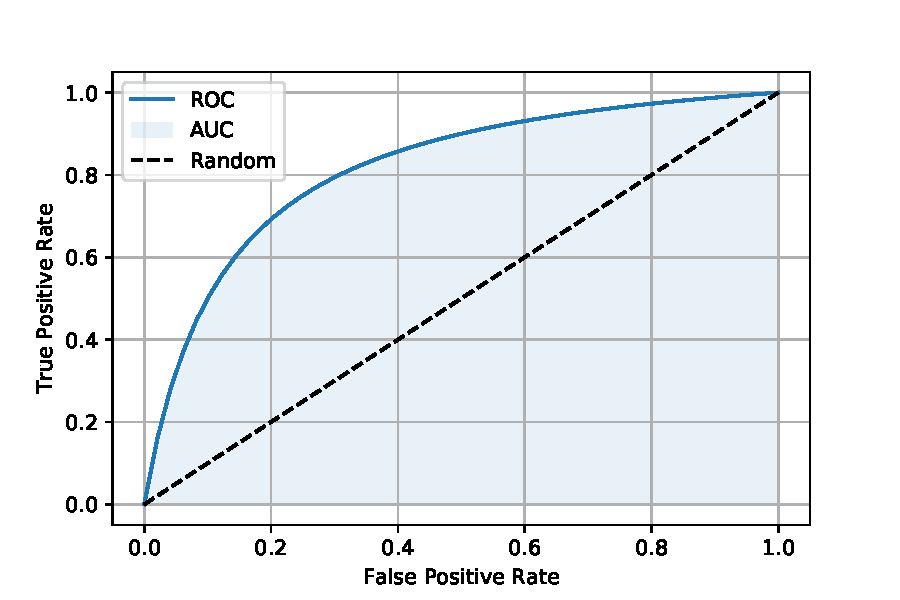
\includegraphics[trim=0 0 0 1cm, clip, width=0.6\textwidth]{contents/figures/Method/AUC-ROC-Curve}
        \end{xblock}
    
    \end{xframe}
    
    \subsection{Model Optimization}
    \begin{xframe}
        \begin{xblock}{Gradient Descent}<.->
            \begin{displayquote}\itshape
                Gradient descent is an optimization algorithm used to minimize a function by iteratively moving in the direction of the steepest descent as defined by the negative of the gradient. 
            \end{displayquote}
            \centering
            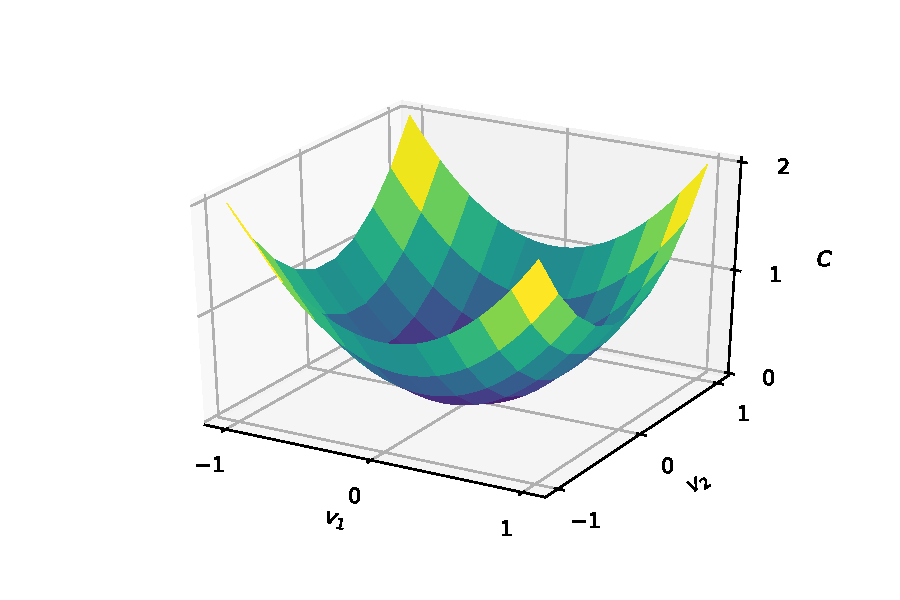
\includegraphics[trim=2.75cm 1cm 0.75cm 1.5cm, clip,width=0.6\textwidth]{contents/figures/Method/Gradient-Descent}
        \end{xblock}
    \end{xframe}
    
    \subsection{PyTorch Implementation}
    
    \begin{xframe}
        \begin{xblock}{Pairwise Distance}
            Compute distances using quadratic expansion
            \[\Vert\z_i-\z_j\Vert^2\equiv\Vert \z_i\Vert^2 + \Vert\z_j\Vert^2 - 2(\z_i\cdot\z_j)\]
        \end{xblock}
        
        \begin{xblock}{Latent Space Positions}
            Compute positions based on $\Z_0$
            \[ \Z_{t-1} + \bmepsilon_t \equiv \Z_0 + \sum_{i=1}^t\bmepsilon_i \]
            \onslide<+->
            Use warm start for autoregressive models
        \end{xblock}
    \end{xframe}
    
    \begin{xframe}
        \begin{xblock}{Estimating Innovations}
            Infer innovations and penalize addition of diffusion
            \[\log\mathcal{L}(\mu, \sigma^2\vert \x) = -\frac{n}{2}\log2\pi - \frac{n}{2}\log\sigma^2 - \frac{1}{2\sigma^2}\sum_{i=1}^n (x_i - \mu)^2\]
            \onslide<+->
            Optimize variance analytically using the MLE of $\sigma^2$
        \end{xblock}
        
        \begin{xblock}{Node Batching}
            Use slices instead of indices for batching
            \onslide<+->
            \begin{center}
                \begin{tikzpicture}
    \matrix (m) [matrix of math nodes,
                 nodes={append after command={\pgfextra{\draw 
                 ($(\tikzlastnode.north west)+(-1mm,0mm)$)
                 rectangle ($(\tikzlastnode.south east)+(1mm,0mm)$);}}},
                 column sep=-0.5pt, row sep=-0.5pt]
    {
        0 & 0 & 1 & 2 & 2 & 3 & 3 & 4 & 4 & 6 & 6 & 7 \\
        2 & 6 & 6 & 5 & 7 & 0 & 2 & 1 & 6 & 4 & 7 & 3 \\
        1 & 1 & 1 & 1 & 1 & 1 & 1 & 1 & 1 & 1 & 1 & 1 \\
    };
    
    \tikzset{every node/.style = {text width=2cm, font=\itshape}}
    \foreach \t [count=\i] in {row, column, value}{
        \node[left of=m-\i-1]{\t};
    }
    
    \begin{pgfonlayer}{myback}
        \xmatfill(1){m-1-1}{m-3-5}
        \xmatfill(1)[gray!40]{m-2-1}{m-3-1}
        
        \xmatfill(1)[gray!40]{m-1-6}{m-3-12}
        \xmatfill(1){m-2-9}{m-2-9}
        \xmatfill(1){m-2-11}{m-2-11}
    \end{pgfonlayer}
\end{tikzpicture}
            \end{center}
        \end{xblock}
    
    \end{xframe}
    
\section{Data}

    \subsection{Synthetic Data}
    
    \subsubsection{Static Data}
    
    \begin{xframe}
        \centering
        \animategraphics[autoplay,width=0.8\textwidth]{12}{contents/figures/Data/Static/Data}{}{}
    \end{xframe}
    
    \subsubsection{Dynamic Data}
    
    \begin{xframe}
        \centering
        \animategraphics[autoplay,width=0.8\textwidth]{12}{contents/figures/Data/Dynamic/Data}{}{}
    \end{xframe}
    
    \subsubsection{Periodic Data}
    
    \begin{xframe}
        \centering
        \animategraphics[autoplay,width=0.8\textwidth]{3}{contents/figures/Data/Periodic/Data}{}{}
    \end{xframe}
    
    \subsection{EU Email Data}
    
    \begin{xframe}
        \centering
        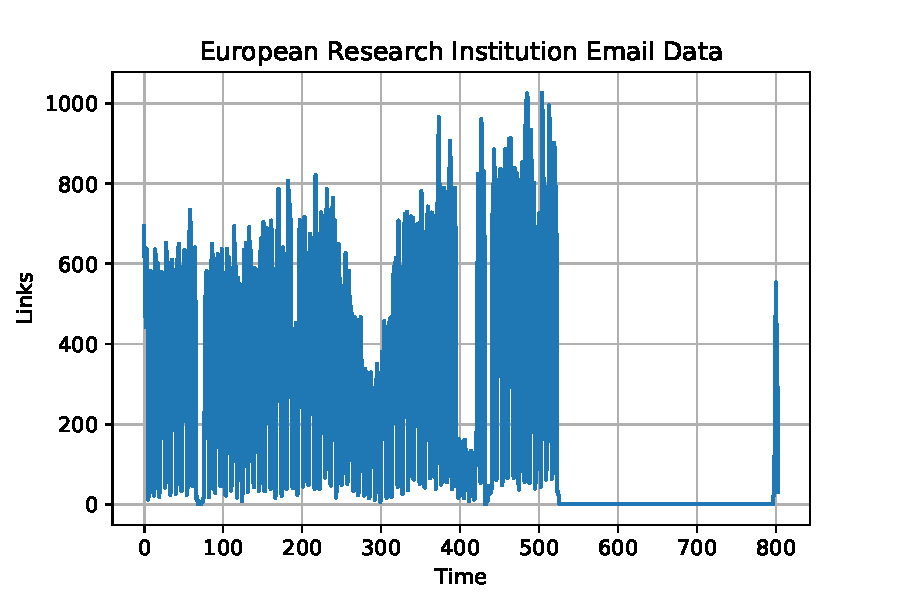
\includegraphics[width=0.8\textwidth]{contents/figures/Data/EUEmail/Links}
    \end{xframe}
    
    \begin{xframe}
        \centering
        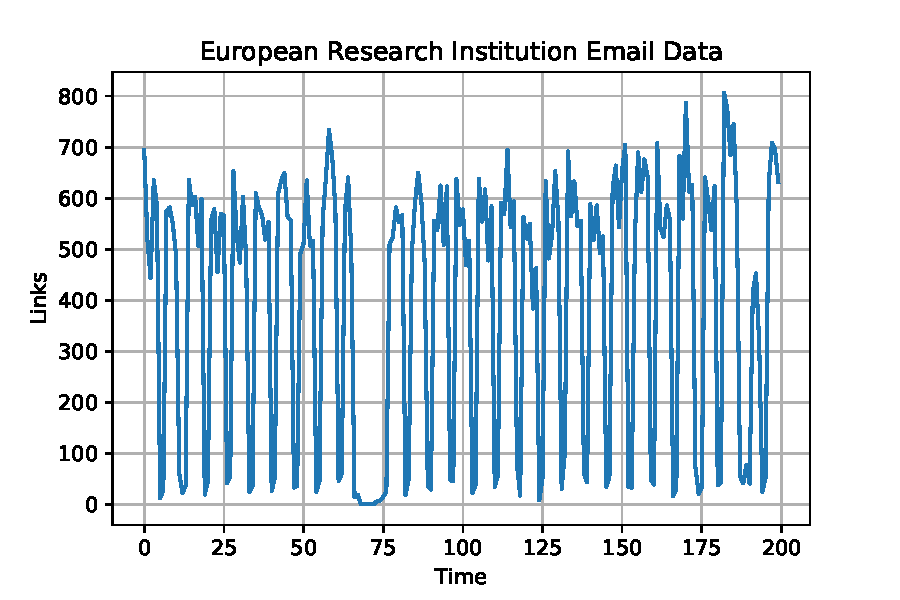
\includegraphics[width=0.8\textwidth]{contents/figures/Data/EUEmail/Links0-200}
    \end{xframe}
    
    \subsection{UC Messaging Data}
    
    \begin{xframe}
        \centering
        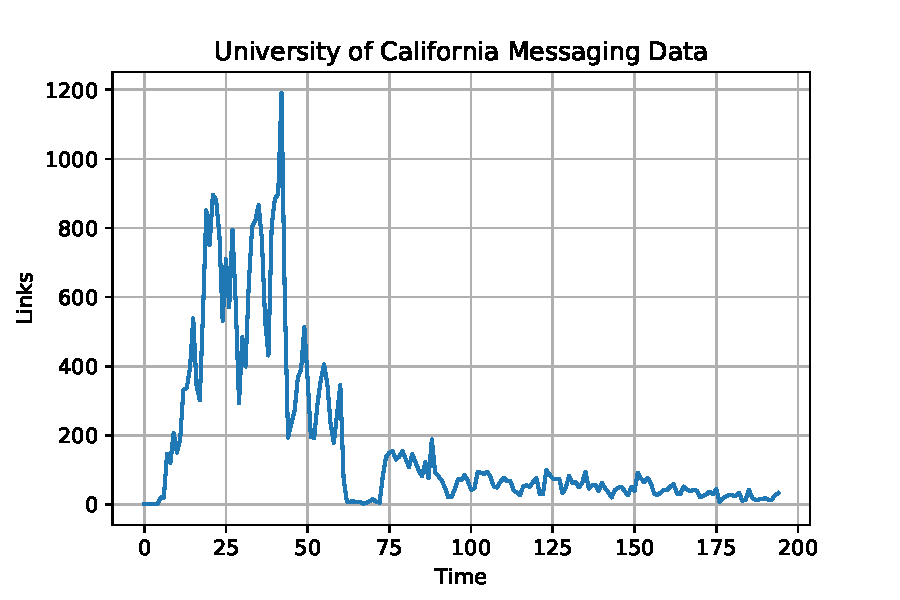
\includegraphics[width=0.8\textwidth]{contents/figures/Data/UCMessaging/Links}
    \end{xframe}
    
    \begin{xframe}
        \centering
        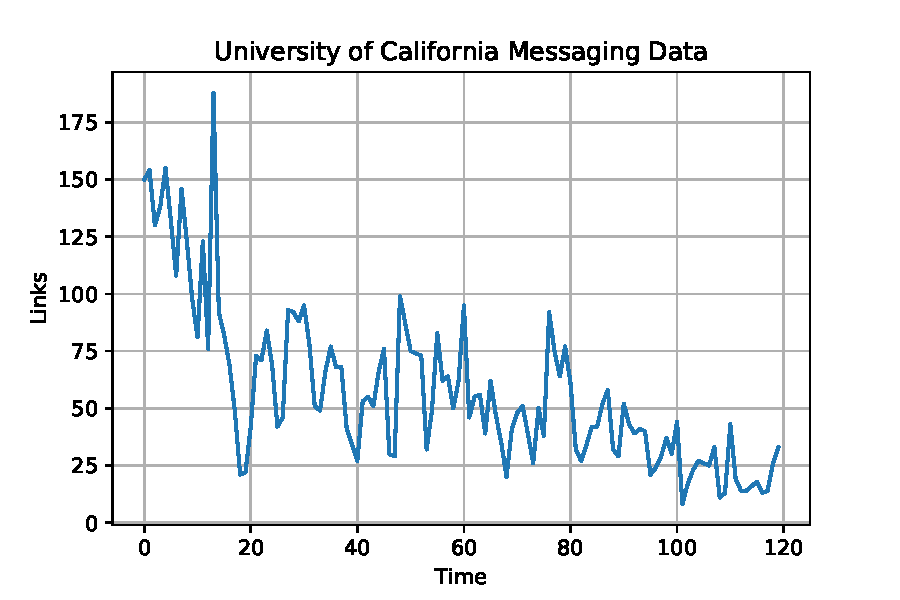
\includegraphics[width=0.8\textwidth]{contents/figures/Data/UCMessaging/Links75-195}
    \end{xframe}
    
\section{Results}

    \subsection{Synthetic Data}
    
    \subsubsection{Static Data}
    
    \begin{xframe}
        \xdouble
            {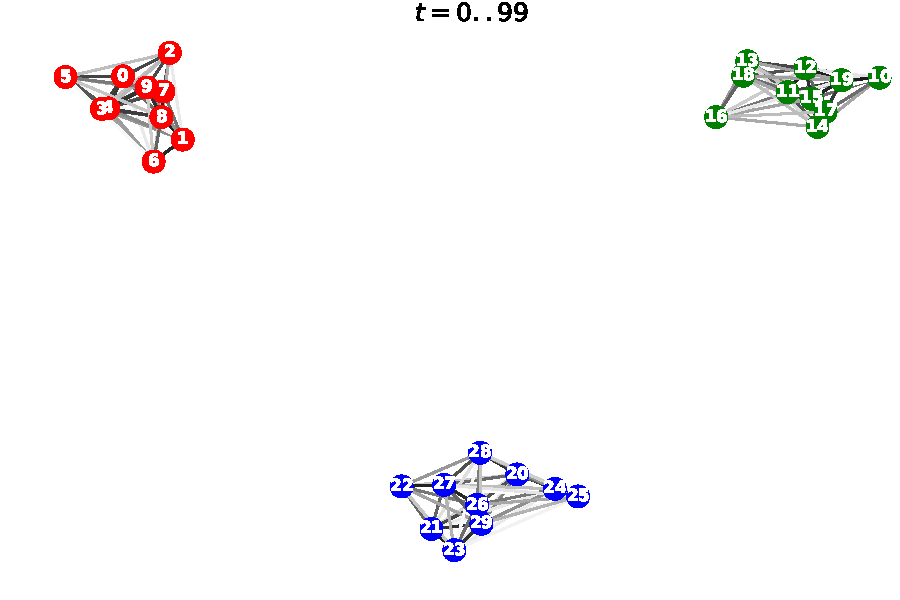
\includegraphics[width=\textwidth]{contents/figures/Results/Static/Proba/StaticModel-AR(1)-Undirected-True}}
            {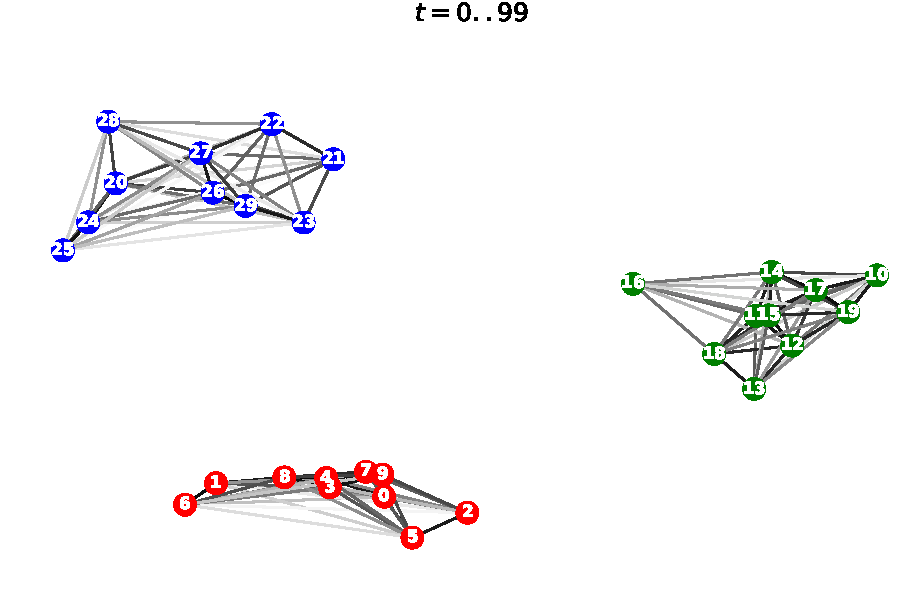
\includegraphics[width=\textwidth]{contents/figures/Results/Static/Proba/StaticModel-AR(1)-Undirected-NoLoss}}
    \end{xframe}
    
    \begin{xframe}
        \centering
        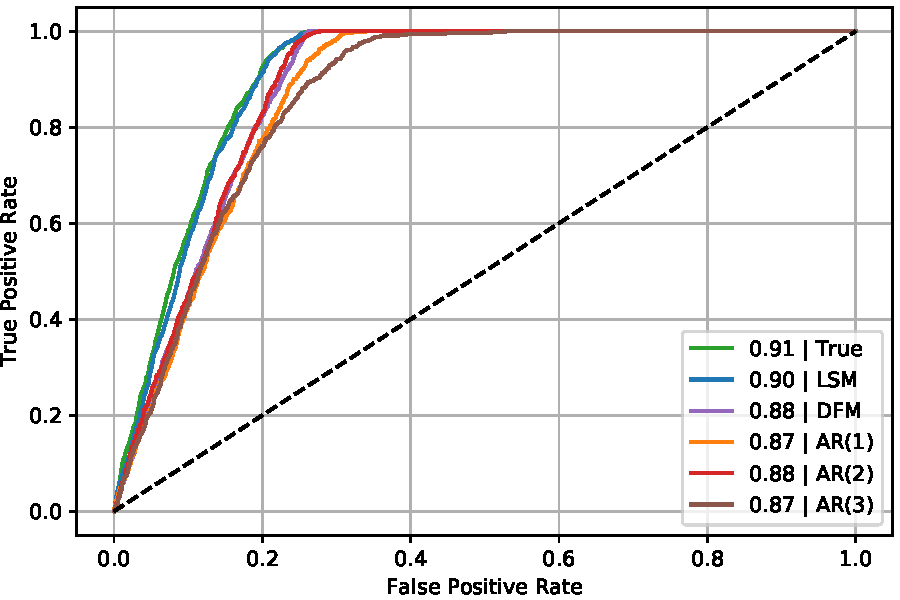
\includegraphics[width=0.8\textwidth]{contents/figures/Results/Static/AUC-Undirected-NL}
    \end{xframe}
    
    \subsubsection{Dynamic Data}
    
    \begin{xframe}
        \xdouble
            {\animategraphics[autoplay,width=\textwidth]{12}{contents/figures/Results/Dynamic/Proba/DiffusionModel-AR(1)-Undirected-True}{}{}}
            {\animategraphics[autoplay,width=\textwidth]{12}{contents/figures/Results/Dynamic/Proba/DiffusionModel-AR(1)-Undirected-GaussianLossNoVar}{}{}}
    \end{xframe}
    
    \begin{xframe}
        \centering
        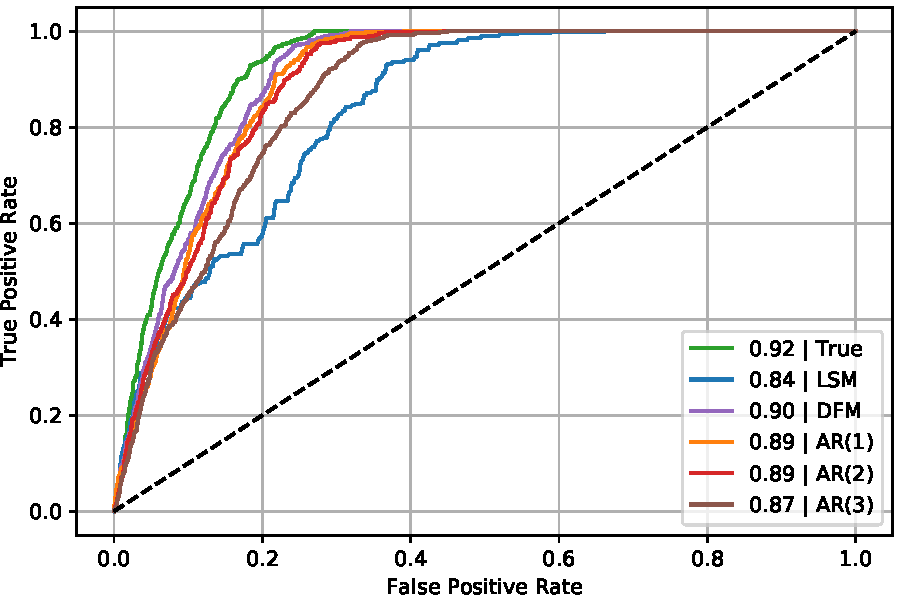
\includegraphics[width=0.8\textwidth]{contents/figures/Results/Dynamic/AUC-Undirected-GNV}
    \end{xframe}
    
    \subsubsection{Periodic Data}
    
    \begin{xframe}
        \xdouble
            {\animategraphics[autoplay,width=\textwidth]{3}{contents/figures/Results/Periodic/Proba/AutoregressiveModel-AR(3)-Undirected-True}{}{}}
            {\animategraphics[autoplay,width=\textwidth]{3}{contents/figures/Results/Periodic/Proba/AutoregressiveModel-AR(3)-Undirected-GaussianLoss}{}{}}
    \end{xframe}
    
    \begin{xframe}
        \centering
        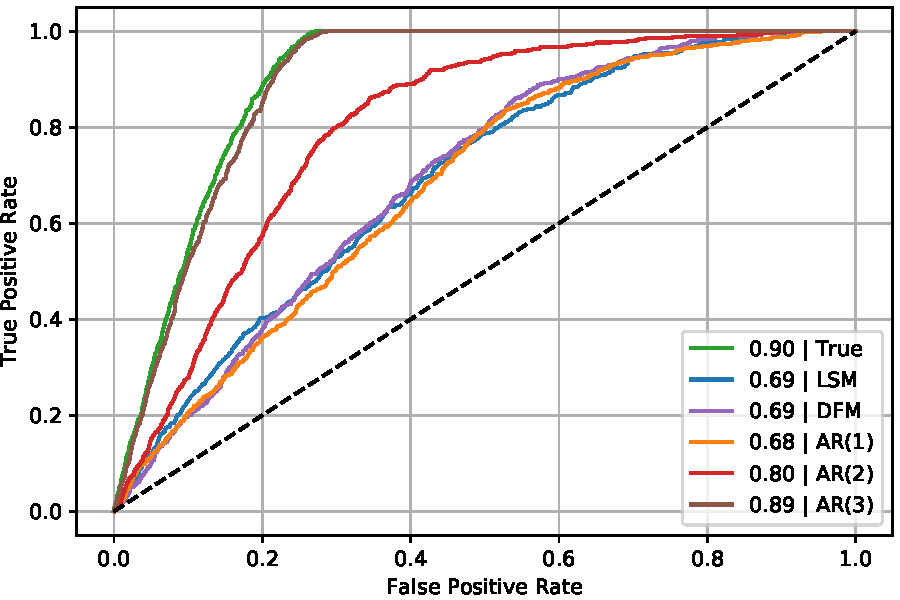
\includegraphics[width=0.8\textwidth]{contents/figures/Results/Periodic/AUC-Undirected-GL}
    \end{xframe}
    
    \subsection{EU Email Data}
    
    \begin{xframe}
        \centering
        \animategraphics[autoplay,width=0.8\textwidth]{6}{contents/figures/Results/EUEmail0-200/Proba/AutoregressiveModel-AR(3)-Undirected-K(2)-GL-1}{}{}
    \end{xframe}
    
    \begin{xframe}
        \centering
        \animategraphics[autoplay,width=0.8\textwidth]{6}{contents/figures/Results/EUEmail0-200/Proba/AutoregressiveModel-AR(7)-Directed-K(3)-GL-1}{}{}
    \end{xframe}
    
    \begin{xframe}
        \centering
        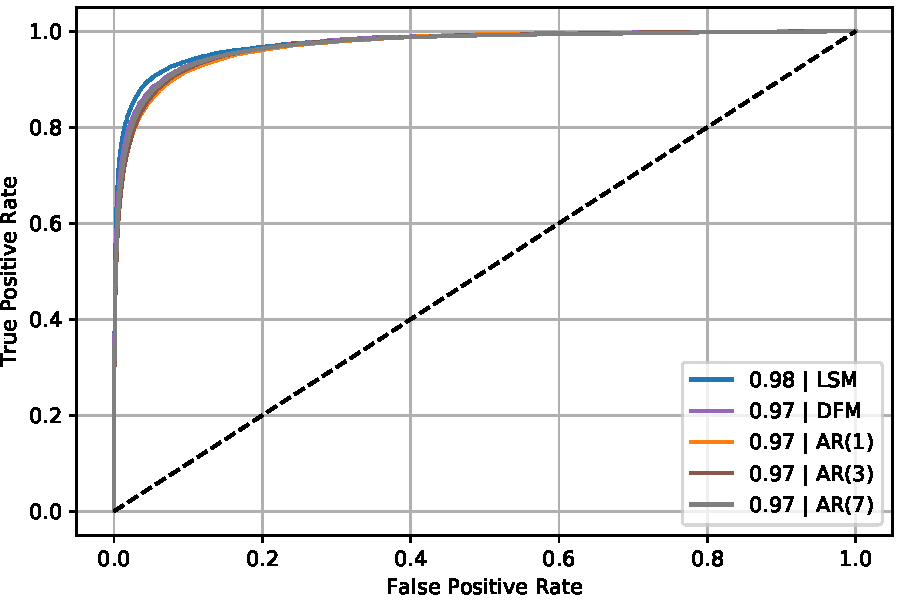
\includegraphics[width=0.8\textwidth]{contents/figures/Results/EUEmail0-200/AUC-Directed-K(10)-GL}
    \end{xframe}
    
    \subsection{UC Messaging Data}
    
    \begin{xframe}
        \centering
        \animategraphics[autoplay,width=0.8\textwidth]{6}{contents/figures/Results/UCMessaging75-195/Proba/AutoregressiveModel-AR(3)-Undirected-K(3)-GL-1}{}{}
    \end{xframe}
    
    \begin{xframe}
        \centering
        \animategraphics[autoplay,width=0.8\textwidth]{6}{contents/figures/Results/UCMessaging75-195/Proba/AutoregressiveModel-AR(7)-Directed-K(2)-GL-1}{}{}
    \end{xframe}
    
    \begin{xframe}
        \centering
        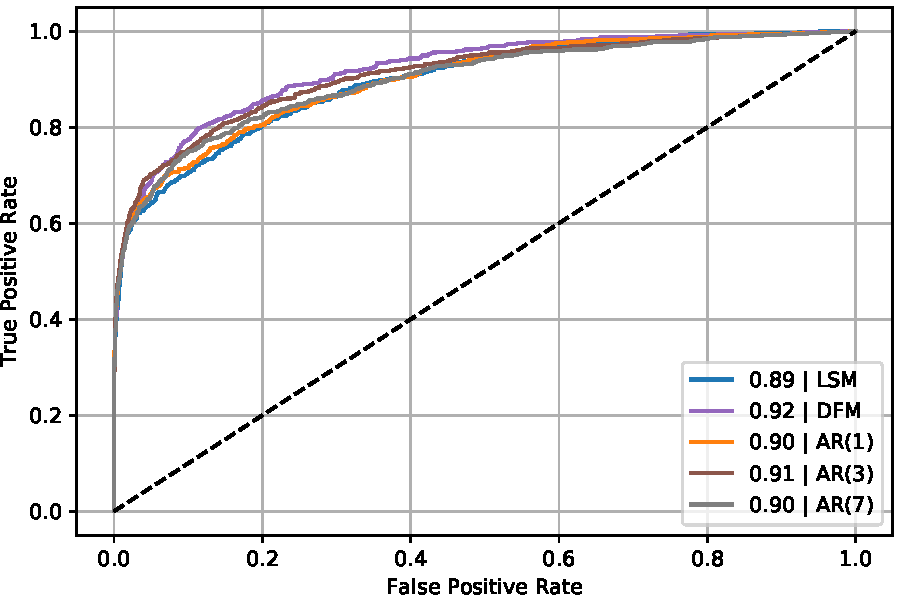
\includegraphics[width=0.8\textwidth]{contents/figures/Results/UCMessaging75-195/AUC-Directed-K(10)-GL}
    \end{xframe}
    
\section{Discussion}

    \subsection{Summary}
    
    \begin{xframe}
        \begin{xblock}{Synthetic Data}
            \begin{itemize}
                \item<.-> Static model better on static data
                \item Diffusion model better on dynamic data
                \item Autoregressive model better on periodic data
            \end{itemize}
        \end{xblock}
        
        \begin{xblock}{EU Email Data}
            \begin{itemize}
                \item<.-> Static model slightly better than dynamic models
                \item No difference between undirected and directed for high-dimensional latent spaces
            \end{itemize}
        \end{xblock}
        
        \begin{xblock}{UC Messaging Data}
            \begin{itemize}
                \item<.-> More difficult to predict overall, possibly due to increased sparsity
                \item Diffusion model slightly better than AR models
                \item Distinct difference between undirected and directed models
            \end{itemize}
        \end{xblock}
    \end{xframe}

    \subsection{Model Variations}
    
    \begin{xframe}
        \begin{xblock}{Static vs Dynamic}
            \begin{itemize}
                \item<.-> Distinction not as prominent for real-life networks
                \item The seemingly periodic EU email dataset was readily modeled by a static model
                \item Dynamic models were beneficial modeling the UC messaging dataset, possibly due to the negative trend
                % \item Datasets 
            \end{itemize}
        \end{xblock}
        
        \begin{xblock}{Autoregressive Order}
            \begin{itemize}
                \item<.-> Important to distinguish between total link activity and per-observation basis
                \item Other datasets should be analyzed to further investigate the effects of the AR order
            \end{itemize}
        \end{xblock}
        
        \begin{xblock}{Undirected vs Directed}
            \begin{itemize}
                \item<.-> Quite different latent representations
                \item Reciprocal and transitive relationships
            \end{itemize}
        \end{xblock}
    \end{xframe}
    
    \begin{xframe}
        \begin{xblock}{$k$-Dimensional}
            \begin{itemize}
                \item<.-> Huge impact on performance
                \item Allows for increasingly complex placement of observations
                \item Two and three-dimensional latent spaces used for visualization
                \item Further analysis should be carried out in terms of the latent dimensionality
            \end{itemize}
        \end{xblock}
        
        \begin{xblock}{Diffusion Penalty}
            \begin{itemize}
                \item<.-> Overfitting without diffusion penalty
                \item Underfitting with Gaussian diffusion penalty on synthetic dynamic data
                \item Insignificant differences between the penalties on real-life networks
                \item Experiment with synthetic dataset based on Laplace distribution
            \end{itemize}
        \end{xblock}
    \end{xframe}
    
    \subsection{Extensions}
    
    \begin{xframe}
    
        \begin{xblock}{Several extensions are possible, e.g.}
            \begin{enumerate}
                \item<.-> \emph{hyperparameter tuning}, analyzing impact of batch sizes and parameter initializations
                \item \emph{parallelization}, performing model optimization on multiple GPUs
                \item \emph{approximate likelihood}, reducing time complexity of calculating the likelihood to $O(N)$ down from $O(N^2)$
                \item \emph{direct AR computation}, avoiding linear scaling with the number of time steps
                \item \emph{GPU validation}, computing AUC scores without transferring data to CPU
                \item and \emph{Procrustean transformation}, removing rotation, translation, reflection and scaling
            \end{enumerate}
        \end{xblock}
    \end{xframe}
    
\section{Conclusion}

    \begin{xframe}
        \begin{xblock}{What has been done?}
            \begin{itemize}
                \item<.-> From three hours with 30 nodes over 23 time steps, to half an hour with almost 2,000 nodes over 120 time steps
                \item A result of using MLE instead of Bayesian inference, facilitating GPU computation
                \item Pairwise distance computation, numerically stable loss, GPU-based batching strategy
            \end{itemize}
        \end{xblock}
        
        \begin{xblock}{What were the results?}
            \begin{itemize}
                \item<.-> Replicated \citeauthor{zangenberg2018a}'s results on synthetic data
                \item Achieved AUC scores above 90\% on two real-life networks
                \item Provided excessive latent space visualizations
            \end{itemize}
        \end{xblock}
    \end{xframe}
    
    \begin{xframe}
        \begin{xblock}{What is the conclusion?}
            Let us recap the initial questions
            \begin{itemize}
                \item \textit{Will a GPU-based framework allow the modeling of large dynamic complex networks for several time steps?}
                \item[] Yes, considering networks with 2,000 nodes as large and 200 time steps as several
                \item \textit{Is a simple AR model sufficient to capture dynamic relations of complex networks, or will the task require more advanced models?}
                \item[] The answer depends entirely on the network in question, such that the thesis will serve as motivation for the reformulated question; \onslide<+-> \textit{How many complex networks is the AR model capable of capturing the dynamic relations of?}
            \end{itemize}
        \end{xblock}
    \end{xframe}
    
\section*{Bibliography}

    \begin{frame}{\strut}{\insertsection}
        \printbibliography
    \end{frame}
    
\end{document}